% THIS IS SIGPROC-SP.TEX - VERSION 3.1
% WORKS WITH V3.2SP OF ACM_PROC_ARTICLE-SP.CLS
% APRIL 2009
%
% It is an example file showing how to use the 'acm_proc_article-sp.cls' V3.2SP
% LaTeX2e document class file for Conference Proceedings submissions.
% ----------------------------------------------------------------------------------------------------------------
% This .tex file (and associated .cls V3.2SP) *DOES NOT* produce:
%       1) The Permission Statement
%       2) The Conference (location) Info information
%       3) The Copyright Line with ACM data
%       4) Page numbering
% ---------------------------------------------------------------------------------------------------------------
% It is an example which *does* use the .bib file (from which the .bbl file
% is produced).
% REMEMBER HOWEVER: After having produced the .bbl file,
% and prior to final submission,
% you need to 'insert'  your .bbl file into your source .tex file so as to provide
% ONE 'self-contained' source file.
%
% Questions regarding SIGS should be sent to
% Adrienne Griscti ---> griscti@acm.org
%
% Questions/suggestions regarding the guidelines, .tex and .cls files, etc. to
% Gerald Murray ---> murray@hq.acm.org
%
% For tracking purposes - this is V3.1SP - APRIL 2009

\documentclass{acm_proc_article-sp}

\begin{document}

\title{An Investigation of the Effects of Mental Fatigue on Programming Tasks'
Performance}

\numberofauthors{2} %  in this sample file, there are a *total*

\author{
% You can go ahead and credit any number of authors here,
% e.g. one 'row of three' or two rows (consisting of one row of three
% and a second row of one, two or three).
%
% The command \alignauthor (no curly braces needed) should
% precede each author name, affiliation/snail-mail address and
% e-mail address. Additionally, tag each line of
% affiliation/address with \affaddr, and tag the
% e-mail address with \email.
%
% 1st. author
\alignauthor
Saurabh Sarkar\\
       \affaddr{Department of Computer Science}\\
       \affaddr{North Carolina State University}\\
       \affaddr{Raleigh, NC}\\
       \email{ssarkar4@ncsu.edu}
% 2nd. author
\alignauthor
Chris Parnin\\
       \affaddr{Department of Computer Science}\\
       \affaddr{North Carolina State University}\\
       \affaddr{Raleigh, NC}\\
       \email{cjparnin@ncsu.edu}
}

\maketitle
\begin{abstract}
Mental fatigue reduces the cognitive and physical performance of people. 
Fatigue has been considered as a crucial issue in different fields like
driving but not in software development. We propose to investigate
how mental fatigue  adversely affects the performance of a software
professional, causing systems developed by them to fail in the long run. We
have tried answering our research questions and validated our hypothesis with
the help of surveys including 311 participants and observing the results
of few user studies. This project is to define the research guidelines to
further investigate different methods to automatically determine the fatigue
level of developers. We can use this information to help developers avoid
their fatigue state to control errors in programming, and thereby aid them to
be more productive.
\end{abstract}

\keywords{Software Engineering, Psychology, Fatigue, Work Environment} % NOT
% required for Proceedings

\section{Introduction}
Fatigue is a physiological state of reduced mental or physical mental
capability \cite{psychology:paul}. It
results from excessive workload(both physical and mental), exhaustion, or
sleeploss. Fatigue is ambiguous in definition. Fatigue (also called
exhaustion, tiredness, and lethargy) \cite{website:wiki-fatigue} is a complex
phenomenon encompassing several physiological and psychological characterisitics
\cite{psychology:paul}. Fatigue can be categorized according to the distinct
effects it has on a person. The inability to perform any physical activities at
the level of one's normal activities is \textit{physical/muscular fatigue}.
\textit{Mental fatigue} is defined as a state of weariness, with a feeling of
boredom/saturation and declines motivation \cite{lauren:defining}. Dull
emotional responses is characterized as \textit{Emotional Fatigue}.
\textit{Skills Fatigue} deals with the inability to perform a certain task at
one's usual capacity. People are susceptible to fatigue that could
potentially hamper our daily activities by affecting our ability to perform and
thus lead to undesirable results.

Mental fatigue is triggered by long and demanding tasks \cite{lauren:defining}.
Exhaustion due to extreme mental and physical work causes performance
degradation in execution of human tasks. Mental fatigue also has a negative
effect on memory and cognitive functionalities and these functionalities play a
vital role in program construction and modeling \cite{schneiderman:interaction}.
Mental fatigue is universal to all software developers
\cite{website:blog-fatigue}. Studies have shown possible relations between
mental fatigue and specific programming tasks such as a program construction,
modeling and debugging \cite{schneiderman:interaction}.

Primary reasons for system failures are due to low performance of developers,
caused by their absentmindedness or exhaustion. Mental fatigue can also lead to
system failures in the long run \cite{rocco:gartner}. In today's competitive
world, software developers are motivated to work hard, and and hence are
involved in numerous projects. Sometimes they work in teams and and at other
times, they work individually on a project. All of this leads to sleep
deprivation that results in exhaustion and tiredness. Several times developers
suffer from psychological diseases which they themselves are not aware of
\cite{website:blog-fatigue}. Developers may make mistakes and therefore
introduce bugs during software development. These mental errors are due to
reduced cognitive functioning like distraction, low decision making power, less
reasoning capabilities, and poor attention and focus \cite{larson:cogFailures}.

Tests \cite{saito:industry} quantify few subjective symptoms of fatigue in
performing general tasks, that relates to programming domain, in Table
~\ref{table:symptoms}.

	\begin{table*}
		\centering
		\caption{Subjective symptoms of fatigue}
		\begin{tabular}{|c|c|l|} \hline
			\textbf{Exhausted \& Drowsy} & \textbf{Mental decline} & \textbf{Incongruity
			in body \& nervous systems}\\ \hline
			Sleepiness&Nervousness&Physical Strength\\ \hline
			Restlessness&Unwillingness&Pain in limbs\\ \hline
			Feeling tired&Lack of focus&Strain in eyes\\ \hline
			Sluggish&Absentmindedness&Dizziness\\ \hline
			Lethargy&Anxiety& \\ \hline
			 &Weariness& \\ \hline		
			\end{tabular}
		\label{table:symptoms}
	\end{table*}

There is not a lot of work done in this problem area, so our approach would be
to create incremental models that can be refined over time with continuous
evaluation of the research. Our contribution intends to define some measurements
for measuring the mental fatigue and analyzing its effect on developers'
performance, which are discussed further in the paper. This is a step towards
working to solve the problem of developers' mental fatigue affecting various
programming tasks in the software development process. In Section 2, we
illustrate the related works in the field of fatigue and what other cognitive
aspects have been researched in programming domain. Section 3 presents how
we define some research questions and how they are answered by the help
of a survey and a formulative study. Here we also discuss the results of our
study and give a detailed analysis of the observations providing a vision of our
research. In Section 4, we discuss how the study can be helpful in the field
of software engineering.

\section{Related Work}
Empirical studies have been conducted in the cognitive aspects 
of software engineering. Khan et. al. \cite{khan:mood} have worked on the effect 
of programmers' moods on the performance of programming debugging, 
which also comes under the umbrella of psychological causes. 
Our approach takes mental fatigue as the psychological factor 
rather than mood and focuses on all programming tasks, not just debugging.
Pimenta et. al. \cite{pimenta:monitor} \cite{pimenta:analysis} have worked on
monitoring and analyzing human performance with respect to computer related
tasks and detailing the effects of fatigue on performance. My proposal is the
extension of this approach by using different ways to analyze the effects of
fatigue and and helping the developer overcome it. Saito \cite{saito:industry}
has worked on assessment of physical fatigue in industries. Several studies have
been conducted to understand the risk of reduced cognitive capability while
driving or performing other physical activities in industries. However, very
little research has been carried out in assessing the risk for programming.
Articles \cite{website:blog-decision} and blogs \cite{website:blog-fatigue}
discuss about the effect of fatigue on the efficacy of developers in tasks like
program understanding, construction, modeling, debugging and decision making.
We believe that industry requires a tool that can aid a programmer in detecting
their state of mental fatigue and help overcome it.

This proposed project is first of the many steps taken in this 
direction, opening a wider scope for more research in the domain.

\section{Methodology}
The approach is to test our hypothesis and then set some research
guidelines to investigate methods to determine fatigue state of developers. In
order to set the research guideline, we have answered few research questions:
\begin{itemize}
  \item RQ1: \textit{How severely and frequently does fatigue impactdeveloperr
  productivity?}
  \item RQ2: \textit{What are the factors that lead to mental fatigue and
  how does it affect a programmer's life?}
\end{itemize}
We conducted a formative study to get answer to these questions.
Additionally, the methodology comprises of a case study to try setting some
benchmark, which includes initial experimental validation using an
instrumentation tool \textit{DevFatigue} (Eclipse plug-in).\\

\subsection{Survey}
In order to validate the hypothesis of mental fatigue deteriorting
performance of developers and to resolve the challenge of
quantifying and measuring fatigue with respect to the programming tasks, we
intend to build a novel model to classify fatigue and relate it. However, to
achieve that, we must set some guidelines on the basis of which we will be able
to quantify and define fatigue. This will help us answer the above mentioned
research questions.

We conducted a survey and received responses from 311 participants. This survey
was distributed with \textit{checkbox.io}\footnote{http://checkbox.io/}.
Participants entered in a draw for three \$50 gift cards. Links to this
survey were posted on reddit groups, Quora, posted in Computer Science Facebook
groups, and emailed out to list servs that were directed towards software developers.
The age distribution of the participants lies mostly between 17 and 74. Around
50\% of the participants lied between the age of 20 to 35, implying that they
are aware of the current trend of the industry and of the work culture followed in
software companiescompanies, while the others are older, implying experience in
software industries. The answers from our respondents helped us gather data
about fatigue and investigate possible detection and alleviation mechanisms. The
survey consists of three parts: questions about sleep habits and fatigue levels,
questions about fatigue and work performance and question about work
habits\footnote{https://github.ncsu.edu/alt-code/fatique/blob\\/master/study/survey.md}.
  
\subsubsection{Results}
The results of our survey show developers' view towards fatigue. It helped
us identify the factors leading to mental fatigue and it's influence on the
performance of any programming task. In addition, several implications allow us
to speculate on the way developers behave when they are in the fatigue state.

Most of the questions were straight forward and objective in nature. We expected
direct conclusions from them. The responses helped us answer the research questions:

\textbf{RQ1:} \textit{How severely and frequently does fatigue impact
programmer productivity?} One of our survey questions was on a sliding scale
asking developers to rate the frequency and severity of the effects of fatigue
according to their personal experience. The responses are shown in Figure
~\ref{fig:sevFreq}. The responses implied that it is not a major issue but an
issue worth looking into. Around 50\% of the respondents thought it is a high
severe problem. 45\%-50\% respondents stated that it occurs to them more often
than not. This answers our first reserach question and motivates us to delve
into the problem of mental fatigue of developers in software industry.

\textbf{RQ2:} \textit{What are the factors that lead to mental fatigue state and
how does it affect a programmer's life?} Based on previous studies
\cite{saito:industry}, both authors came up with some factors that might lead to
mental fatigue. We asked the respondents to choose all the factors they think
are correct. We ranked the factors according to the responses we received
[Figure: ~\ref{fig:factors}]. \textit{Stress} and \textit{sleepiness} are the
most voted factors, which validates our definition of mental fatigue in
programming tasks', that triggers from sleepless nights and day-long works.
Physical activities sometimes play a role in triggering exhaustion as well. The
responses supports the work of Khan et. al. \cite{khan:mood} regarding the
effect of programmers' moods on the performance of programming debugging.

To identify the effects of mental fatigue, we focused on a single survey
question:
\textit{Do you feel when you are tired that it influences your work? If yes,
what are some examples?}
Both authors randomly selected 30 responses to this question in order to
identify initial reasons in examples. We used an
online\footnote{https://conceptcodify.com/} open card sort to group the
responses to this question into categories. Card sorting is a technique used to
create mental  models and define taxonomies from data \cite{begel:cards}.
Problem label clarifies the theme behind their reasons. We repeated the exercise
twice, once individually and the next time together. We compared the labels and
finalized Seven labels. The inter-rater agreement score was 21/30 responses.
Mostly the disagreement was between \textit{Productivity} \& \textit{Performance} and
\textit{Mental Work Set} \& \textit{Motivation}. The confusion between
Productivity and Performance was due to the overlap in the definitions. We
define Performance as the speed of completing a task and Productivity as the
completion of a task, to help us sort better.

Although all the factors are some what related to each other. But, it can be
seen in the responses [Figure: ~\ref{fig:influence}], that respondents think
that mental fatigue affects Performance the most. This conclusion can be considered
as one of the research guidelines. We have conducted some studies to validate
this hypothesis and and reached some conclusions in the following sections.

   \begin{figure}
	\centering
	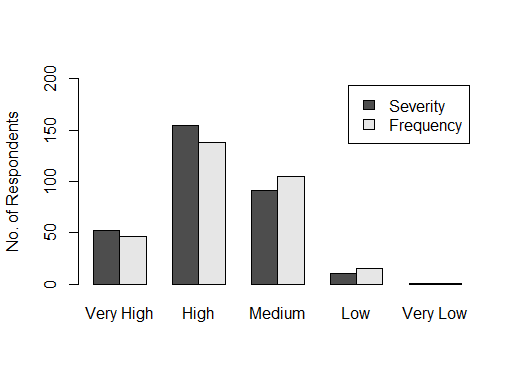
\includegraphics[width=0.5\textwidth,natwidth=517,natheight=382]{sevFreq.png}
	\caption{Severity \& Frequency of fatigue.}
	\label{fig:sevFreq}
   \end{figure}
   \begin{figure}
	\centering
	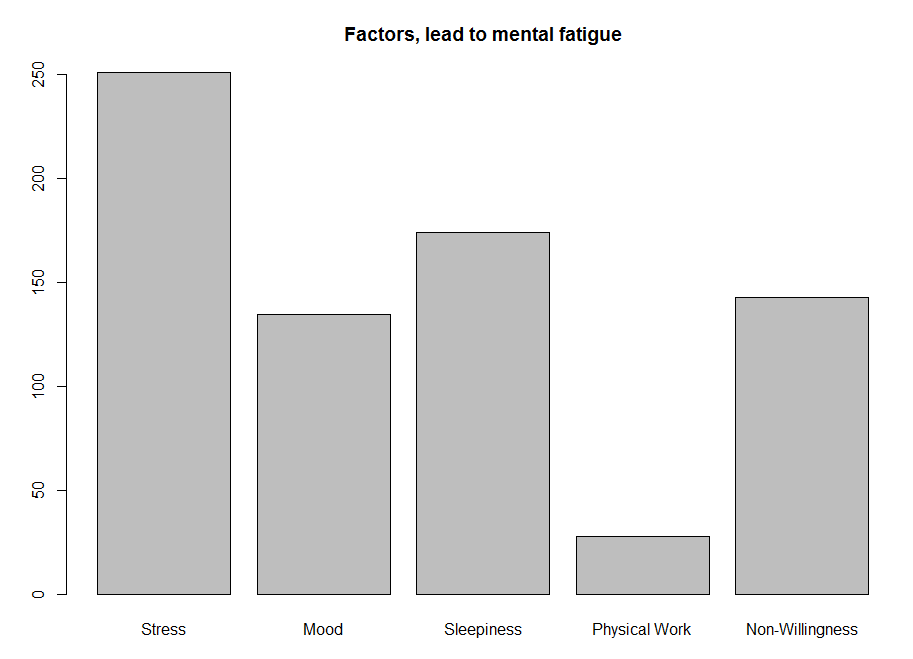
\includegraphics[width=0.5\textwidth,natwidth=1241,natheight=744]{factors.png}
	\caption{Factors leading to mental fatigue.}
	\label{fig:factors}
   \end{figure}
   \begin{figure}
	\centering
	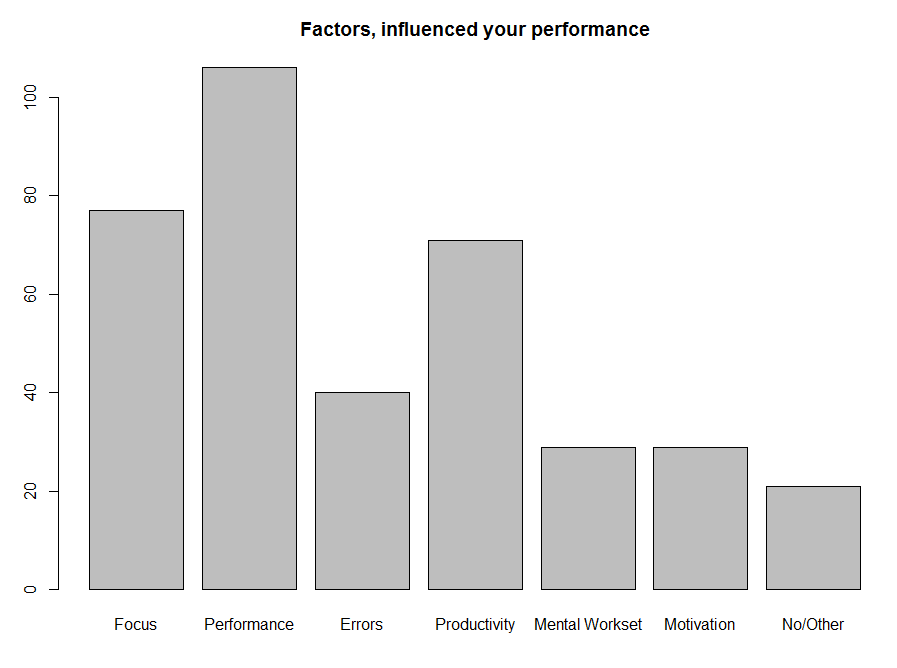
\includegraphics[width=0.5\textwidth,natwidth=1242,natheight=749]{influenced.png}
	\caption{Factors influencing the programming tasks.}
	\label{fig:influence}
   \end{figure}
   
\subsubsection{Threats to Validity}
Although our survey study provides data on fatigue and its detrimental effects
as seen by programmers, there are several threats to validity that should be
considered when interpreting our results. First of all, the survey was not
controlled and included large age group people from 17 to 74. The survey was
posted on various groups assuming that those groups are mostly accessed by
software developers but there was no control over the population. There might be
people from different roles of software industry who might have different and
conflicting opinions. In the responses, there were some respondents as well who
answered that fatigue is not an issue. As all the fields of the responses were
not mandatory, so some responses were blank. In such a scenario, one cannot be
sure that the other fields were answered honestly by such respondents. These
type of threasts are mostly common in case of online surveys but a positive fact
about the analysis here is that the authors were not biased towards the
responses because \textit{checkbox.io} masks the data with anonymous user
details before providing the data.

\subsection{Observation}
To investigate the usefulness of identifying fatigue during programming tasks
and recognizing its impact on the performance, we evaluated the outcome of the
survey study by conducting some other empirical studies of developers.

We implemented a plug-in for the Eclipse IDE.
DevFatigue\footnote{http://www4.ncsu.edu/~ssarkar4/fatigue/eclipse/updatesite/}
is an activity tracking plug-in for Eclipse. It is an extension of
Rabbit\footnote{https://code.google.com/p/rabbit-eclipse/\label{rabbitNote}}.
Like Rabbit, it works in the background with Eclipse and tracks all the
activities you perform. It only tracks the actions when Eclipse is active. And
logs the data in XML (human readable) format at specific location.

The Rabbit features can be referred to on its official
site\footnotemark[\ref{rabbitNote}].\\
Additional features in DevFatigue:
\begin{itemize}
	\item User Activity - The typing speed (key board usage) of the user with
	respect to a time period.
	\item Focus Events - The activities related to keys and mouse usage, like Key
	Up, Key Down, Mouse Clicks, Mouse Velocity, etc. with specific to time period.
	\item Project Events - Information regarding the projects like 'imports', and
	commands used with respect to time period.
\end{itemize}
The architecture of the proposed framework is the extension of the frameworks
used in some of the previous studies \cite{pimenta:analysis}. The framework
collects biometrics, specifically keystroke and mouse dynamics, that will
help in detection and classification of degradation in performance, which can
be an effect of fatigue. We are trying to collect the data in a non-intrusive
and dynamic way and the indicators of mental fatigue recorded by DevFatigue are
in Table 
  	\begin{enumerate}
   		\item Keydown Time: time spent between two consecutive key down and key up
   		events.
   		\item Errors per Key Pressed: number of times a correction is made per key
   		pressed.
   		\item Mouse Velocity: velocity of the cursor.
   		\item Mouse Acceleration: acceleration of the mouse.
   		\item Time between Keys: time spent between two consecutive key up and key
   		down events.
   		\item Time between Clicks: time spent between two consecutive mouse up and
   		mouse down events.
    \end{enumerate}
All the above mentioned indicators have been proved useful in previous studies
\cite{pimenta:monitor} \cite{pimenta:analysis}. These indicators are
collected in a specific time span and provide us information we need to analyze
the working patterns of the users and to infer whether the programmer is
fatigued or not.

\subsubsection{Hack-a-thon}
Overnight programming ccompetitions are always motivational and provide a
platform for developers to work towards solving a problem. A hackathon is a
coding event where computer developers collaborate in building a software
product. LexisNexis organized a fall hack-a-thon on 23rd Oct 2014. We asked the
participants to take part in our study. All of the participants were graduate
students of the Computer Science department at North Carolina State University
(hereafter refered as NCSU).

Of the 13 participants invited to participate in the study, only 2 participants
finished the study and turned in the data by DevFatigue. We collected data using
the log files dumped by DevFatigue, and a post-study questionnaire [Table
~\ref{table:question}].
	\begin{table}
		\centering
		\caption{Post-Hackathon Questionnaire}
		\begin{tabular}{|p{1cm}|p{3cm}|} \hline
			S.No.&Questions\\ \hline
			Q1 & Age?\\ \hline
			Q2 & Any industrial experience?\\ \hline
			Q3 & How would you rate the quality of your code in a scale of 1 to 10, 1
			being the least? \\ \hline
			Q4 & What factors do you think might have affected your performance? \\
			\hline Q5 & Hours slept/rested during the hack-a-thon? \\
			\hline Q6 & Do you think you could have done better, if you had proper rest
			in between? \\ \hline Q7 & Did you win? \\
			\hline
		\end{tabular}
		\label{table:question}
	\end{table}
	
	\begin{figure*}
		\centering
		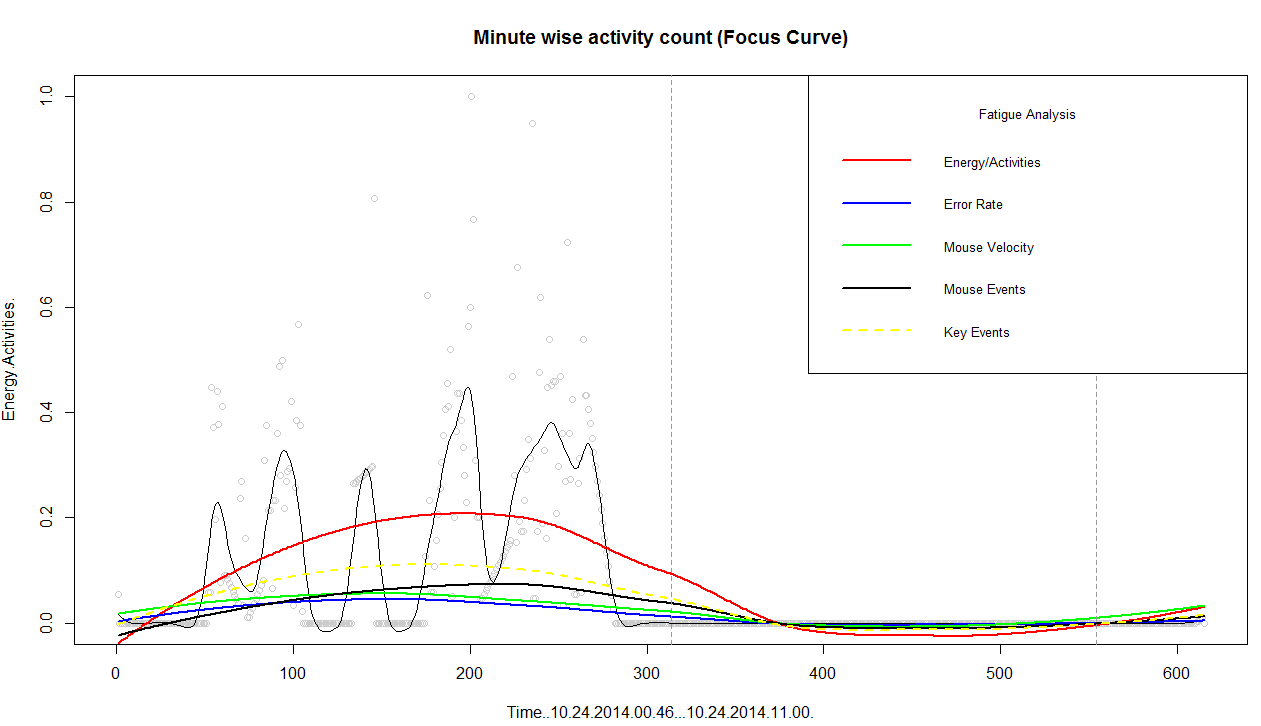
\includegraphics[width=1\textwidth,natwidth=1261,natheight=726]{focusCurveHack.png}
		\caption{Focus Curve - Hack-a-thon Data.}
		\label{fig:hackUser}
  	\end{figure*}
We intended to come up with a focus curve [Figure 6] that can show some working
pattern of the user and build a model based on the data collected to classify
fatigue depending on the user's activities. In our analysis, we defined
\textit{Energy} as the number of activities performed in a time span.
The graph in Figure ~\ref{fig:hackUser} shows the working pattern of a user from
the Hack-a-thon. The corresponding curves are specified by different colors. The
block surrounded by vertical dotted lines represent the sleeping time as shared
by the participant. We can observe that all the features are diminishing while
approaching the sleep time. We observed that the coorelation of Energy with
other features were significant [Table ~\ref{table:question}].
	\begin{table}
		\centering
		\caption{Spearman Correlation Coefficient of features with Energy}
		\begin{tabular}{|c|c|l|} \hline
			Feature&Score\\ \hline
			Key Error & 0.5247477\\ \hline
			Mouse Velocity & 0.6903078\\ \hline
			Mouse Events & 0.7084381\\ \hline
			Key Events & 0.690758\\ \hline
			Navigation & 0.6464797\\ \hline
		\end{tabular}
		\label{table:question}
	\end{table}
	
The results were promising and gave us the motivation to continue our study. Due
to lack of more sessions we could not derive a relation between different
working patterns of the participant. Hence, we decided to analyse a data set
where we could find more working sessions of a user. We used UDC (Usage Data
Collector) data set that was available to us.\\

\subsubsection{Usage Data Collector}
UDC\footnote{https://eclipse.org/epp/usagedata/} is a framework in Eclipse to
collect usage data information. UDC data sets contain the activity information
of a particular user, specifically the commands used through a session. More
than 50000 records were available for each user. We decided to just analyse
100 days sessions of 2 users. The sessions were short but comparative to other
sessions.
For each user, we collected the energy score and calculated the average energy
score of a particular session (time span). Our baseline approach was to
compare day time sessions to night time sessions, with the assumption that one
of the session set would have a fatigue effect. We used a threshold of 20
minutes to declare a session different from another. Users show similar working
patterns on same days of the week. For comparing sessions, firstly, we
considered pairing the scores by day of week. Secondly, we considered session
time as the other comparing feature. We paired similar timed sessions. Finally,
before processing the data set we normalized all the energy sessions to
half-an-hour sessions. We used student's t-test (two tailed) and Cohen's d test for
statistically analysing how each session is different from another session. The null
hypothesis considered is: H\_0: The energy level of day time sessions would be
similar to night time sessions of a user. H\_1: The session durations of day
time sessions would be similar to night time sessions of a user. For each set of
samples compared, the test returns a p-value, with a small p-value suggesting
that it is unlikely that hypothesis is true. Thus, for the test whose p-value <
$\alpha$ the difference is considered to be statistically significant, i.e.
hypothesis is rejected. In this work a value of $\alpha$ = 0.05 is considered, a
standard value generally accepted by research.
	\begin{table}
		\centering
		\caption{Statistical analysis of hypothesis depending on different sessions of
		user} \begin{tabular}{|c|c|l|} \hline
			User&Hypothesis&p-score\\ \hline
			1&H\_0 & 0.001663433\\ \hline
			&H\_1 & 0.19836863\\ \hline
			2&H\_0 & 0.959305717\\ \hline
			&H\_1 & 0.331089607\\ \hline
		\end{tabular}
		\label{table:day/night}
	\end{table}
Table ~\ref{table:day/night} details each hypothesis and its corresponding
p-score. The H\_0 is rejected as its p-score < $\alpha$ for one user, but not
for the other. The rejection of our hypothesis states that there are difference
in energy level in day and night sessions. H\_1 is accepted for both the users
but the score makes us think again about the possibility that it might be
rejected for some other sessions. We have compressed the data before processing first by
averaging it for a time session and then normalizing, that might have lost some
low level information.

The analysis in case of UDC data had some limitations, we had just one
feature data, i.e. energy level (activities). Overall the results are
interesting to warrant further inspection by using finer data sets and feature sets.

\subsubsection{In class study}
Dr. Parnin is teaching CSC 510 Software Engineering in Fall 2014 at NCSU. Most
students in the course have some experience with coding. Dr. Parnin
asked the students to install DevFatigue and let it track their activies on
Eclipse, for a couple of weeks. In addition, we asked them to log their daily
sleep hours.
Of the 100 students enrolled in the course, 19 students responded for the extra
credit offered.
The data shared by the students had more than one session log and the logs
contained detailed time-stamps. We calculated more features and their
correlation coefficients and found them significant with respect to energy
level. According to sleeping time reported by the students, we compared
different sessions of which one can be assumed to be more fatigued than the
other.

\begin{itemize}
  \item \textit{Time between Keys}: Spearman Correlation = 0.7032088\\
  We observed the time between keys of two sessions and compared their
  distribution through out the session by taking the frequency of the time in
  milliseconds. The comparison can be seen in Figure ~\ref{fig:keys}. We
  observed that in a normal session, the short delays covered around 93\% but in
  a fatigued session, the short delays just covered around 85\% and the others
  were long delays. We categorized short delays as 1 to 2000
  milliseconds. We can conclude that under the state of mental fatigue,
  the time between keys increases eventually.
  \begin{figure}
	\centering
	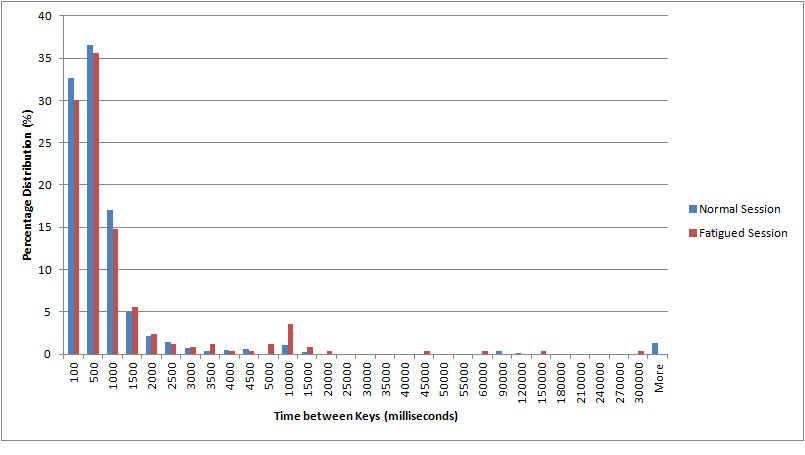
\includegraphics[width=0.5\textwidth,natwidth=805,natheight=455]{timebwkeys.png}
	\caption{Time between keys distribution difference between a normal and a
	fatigued session.}
	\label{fig:keys}
   \end{figure}
  \item \textit{Time between Clicks}: Spearman Correlation = 0.737913\\
  The first thing which we observed were that there were more mouse events
  (clicks, scrolls, and navigations) in fatigued session than normal session.
  The other observation was that, in fatigued session the durations were
  in the same time cluster from 10000 to 30000 milliseconds mostly,
  whereas in normal session it was scattered. We can conclude that in fatigued
  state user demonstrates a sluggish mouse usage and it remains constant
  through out the session and usage of mouse is higher compared to that of
  keys in fatigued sessions.
  \item \textit{Mouse Velocity and Acceleration}\\
  Mouse events in a normal session is less than that of fatigued session
  as mentioned above. Here we have noticed an opposite behavior as of time
  between clicks. Velocity and Acceleration in normal session is around the same
  cluster of speed, but in case of a fatigued session it is scattered. We cannot
  have a definite conclusion here, but the observation states that in case of
  fatigue, a user demonstrates more mouse activity and the speed is random but
  in a normal session his speed is defined.
\end{itemize}

\section{Conclusion \& Future Work}
The study of mental fatigue, including its causes and symptoms, is traditionally
supported by data collected through instrumentation, self-reporting mechanisms
(generally questionnaires) or, more recently, through the use of physiological
sensors. To comprehend the mental fatigue of software developers we conducted a
survey and card sort to catalog factors that lead to fatigue. This study
resulted in answering two of the many research questions related to fatigue
in software development. The survey helped us figure out the factors which are
affected by fatigue and the next step would be to help detect those factors and
help developers to overcome the fatigue state. It could be achieved by various
alerts, screen freezes or even suggesting
Pomodoro\footnote{http://en.wikipedia.org/wiki/Pomodoro\_Technique} technique.
The research is to conduct, monitor, and analyze data in a non-invasive and
non-intrusive way and present the results in a cordial manner. We hope this
paper will encourage similar approaches for finding out how to alleviate mental
fatigue. The results of the conducted formative studies motivates us to delve
further to find more evidence to support our hypothesis.\\
Our research aims to help developers avoid their fatigue state to control
errors in programming, and eventually aid them for a better productivity. The
application would be most suitable for the software industry. We have a lot of
different programming tasks in an industry and fatigue might affect the
performance/productivity of any of those activities. Thus, we will try
conducting some studies on the real environment programming activities.
To check the relation between mental fatigue and performance, we plan to review
bug and code logs. Our research would be taking the following factors into
consideration: working scenarios and behaviors. Smith et. al.\cite{smith:coffee}
studied the effects of intake of coffee on alertness and performance. Coetzer
and Richmond \cite{richmond:team} performed an empirical analysis on working in
teams and its relation to performance.\\
The survey contained many other questions such as asking developers about their
coping strategy under the fatigue state. Future work would include coping
mechanism for fatigue. With the increased interest in the behavior of software
developers, more research should be carried out to identify the adverse effects
of mental fatigue on software development.

\section{Acknowledgement}
Thanks to the CSC510 class at North Carolina State University for
their participation throughout the process of developing this research.
I would like to thank the Alt-Code Group for their support and reviews of the
paper.

%
% The following two commands are all you need in the
% initial runs of your .tex file to
% produce the bibliography for the citations in your paper.
\bibliographystyle{abbrv}
\bibliography{doc}  % sigproc.bib is the name of the Bibliography in this case
% You must have a proper ".bib" file
%  and remember to run:
% latex bibtex latex latex
% to resolve all references
%
% ACM needs 'a single self-contained file'!
%
\balancecolumns
% That's all folks!
\end{document}
